\chapter{Cloud Capacitor}
\label{chap:capacitor}
% ----------------------------------------------------------
A fim de confirmar as hipóteses de eficácia e eficiência do emprego do Processo
de Avaliação de Capacidade descrito no capítulo anterior, bem como da técnica de
Inferência de Desempenho e das Heurísticas de Seleção que dão suporte a esse Processo, 
criamos uma implementação concreta de sua especificação na forma de uma biblioteca
extensível e de um sistema computacional que demonstra seu funcionamento fazendo
a avaliação de uma aplicação real em um provedor de nuvem de infraestrutura.

Demos o nome de CloudCapacitor à biblioteca, implementada como uma \emph{gem} da
linguagem Ruby~\cite{ruby}. Desenvolvemos o sistema computacional Capacitor Web 
para ser uma interface visual para a utilização do CloudCapacitor, usando 
o \emph{framework} Ruby on Rails~\cite{rails}.  

Descrevemos a seguir os detalhes da implementação de cada um e como ambos se
relacionam para oferecer ao usuário a experiência da avaliação de capacidade
de baixo custo e alta precisão prevista pelo Processo proposto, com uma interface
amigável e de fácil utilização.

\section{CloudCapacitor}
CloudCapacitor é uma biblioteca para criação de sistemas de avaliação de 
capacidade em ambientes de nuvem de infraestrutura como serviço. É a implementação
completa da especificação do Processo de Avaliação de Capacidade do 
Capítulo~\ref{chap:processo}, permitindo que sejam customizadas as atividades 
definidas pelo Processo como pontos de extensão, como as Estratégias de Avaliação
e o disparo e controle da execução da Aplicação sob Teste.

Vamos iniciar a apresentação do CloudCapacitor pelas classes que compõem a biblioteca
e suas responsabilidades. Em seguida, veremos como CloudCapacitor auxilia 
desenvolvedores de software na criação de sistemas de avaliação de capacidade,
mostrando o fluxo de utilização da biblioteca através de sua interface de programação.
Depois, falaremos sobre alguns detalhes de implementação da biblioteca, como 
a solução para representação do Espaço de Implantação e seu papel na execução do
Processo de Avaliação de Capacidade. Por fim, apresentaremos os pontos de extensão
da biblioteca, notadamente como implementar um Executor, a classe responsável pelo
controle de execução da Aplicação sob Teste, e como sobrescrever a Estratégia de
Avaliação fornecida pela biblioteca a fim de alterar seu comportamento padrão.

Para concluir a apresentação do CloudCapacitor, será mostrada a saída de dados
fornecida pela biblioteca com as Configurações capazes de executar a
Aplicação sob Teste em cada uma das Cargas de Trabalho respeitando o SLA definido.

\subsection{Classes e Responsabilidades}
\label{subsec:classes}
CloudCapacitor é formado por um conjunto de classes que, juntas representam os
componentes envolvidos na avaliação de capacidade de aplicações em ambientes de
nuvem, de acordo com os conceitos e o Processo definidos anteriormente, nos
Capítulos~\ref{chap:formalizacao} e~\ref{chap:processo}. A Figura~\ref{fig:classes}
mostra as principais classes cujas responsabilidades e cooperação levam ao 
resultado final de uma Avaliação. 

Ao utilizar a biblioteca CloudCapacitor na construção de um software para avaliação
de capacidade, o desenvolvedor tem à sua disposição uma classe principal, chamada
\emph{Cacitor}. Essa classe fornece o fluxo principal do Processo de Avaliação, com todos
os seus pontos de decisão e de extensão.

\begin{figure}[htb]
  \caption{\label{fig:classes}Principais classes que compõem o CloudCapacitor e suas relações}
  \begin{center}
    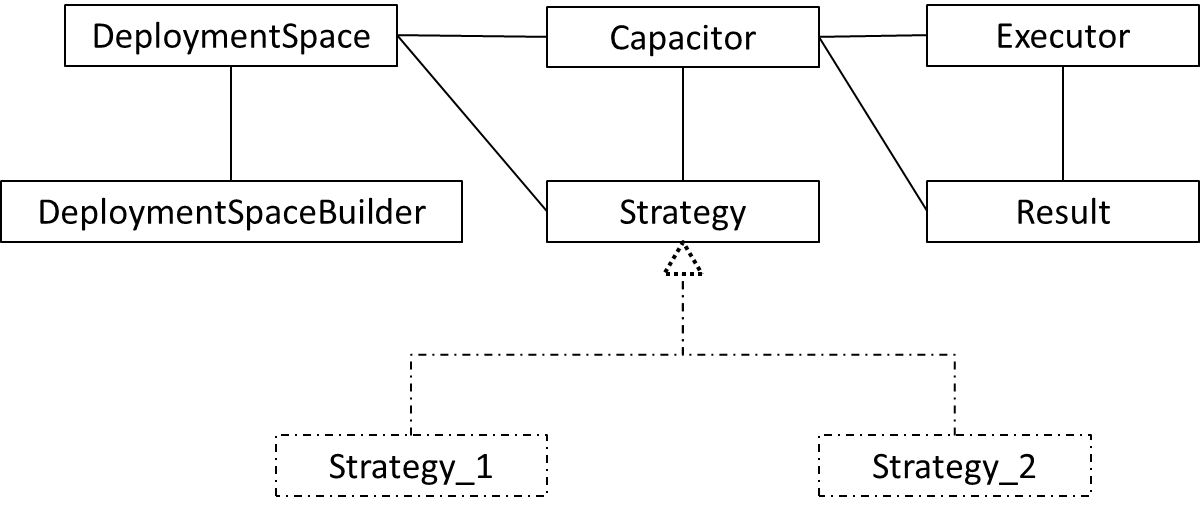
\includegraphics[scale=0.75]{img/CapacitorClasses}
  \end{center}
\end{figure}

Entre os pontos de extensão, destacamos o uso da classe \emph{Strategy}. Como 
vemos na Figura~\ref{fig:classes}, essa classe é fornecida pela biblioteca e a
notação de linhas pontilhadas denota a sua possibilidade de especialização, onde,
sobrescrevendo alguns de seus métodos, é possível criar Estratégias com comportamento
diversificado.

A classe \emph{DefaultExecutor} é o outro ponto de extensão oferecido pela biblioteca.
Porém, neste caso, o desenvolvedor deve mandatoriamente implementar uma subclasse
que forneça a lógica necessária ao controle da execução do teste de desempenho.
Na figura, a classe a ser implementada pelo desenvolvedor é representada com o 
nome de \emph{RealExecutor}.

Para que a Avaliação de Capacidade possa ser efetuada, a classe \emph{Capacitor}
deve conhecer o resultado de cada execução da Aplicação sob Teste, de modo que
possa tomar as decisões corretas na indicação das Configurações Candidatas e
Rejeitadas. Esses resultados são encapsulados na classe \emph{Result}, cujos 
objetos são fornecidos pela subclasse responsável pela execução dos testes de 
desempenho.

E, finalmente, durante a execução da Avaliação de Capacidade, a classe \emph{Capacitor} 
precisa ter conhecimento do Espaço de Implantação disponibilizado. Essa é a 
responsabilidade da classe \emph{DeploymentSpace}, que implementa uma estrutura 
de dados em memória para representar os diversos Níveis de Capacidade formados 
entre as Configurações. A construção dessa estrutura é responsabilidade da classe 
\emph{DeploymentSpaceBuilder}, que contém os algoritmos necessários à preparação 
do grafo usado para navegação pelos Níveis de Capacidade. 

***RASCUNHO***
CloudCapacitor
OK  Diagrama de Classes (UML) / Arquitetura de Componentes
OK  Enumeração das classes e suas responsabilidades
  Fluxo de utilização da biblioteca (caixa preta, interface com o Capacitor)
  Especificação e Carregamento do Deployment Space
  Executor - Implementação
  Estratégia - Descrição da interface
  Estratégia - Como sobrescrever (Gof Strategy Pattern)
  Apresentação do resultado da avaliacao
Capacitor Web
  Apresentação da interface de entrada
  Resultados
  Trace
  Full Trace
Resumo e transicao para o proximo capitulo
***RASCUNHO***



PorémAo instanciar um objeto da classe Capacitor, o desenvolvedor deve atribuir  
Por padrão, o CloudCapacitor oferece uma Estratégia de Avaliação que implementa 
uma lógica simples para as Heurísticas de Seleção de Configurações definidas no
capítulo anterior. Essa lógica pode ser facilmente sobrescrita conforme a necessidade
do usuário ou o perfil da Aplicação sob Teste.


****RASCUNHO
\subsection{Heuristicas}
Para que uma Heurística de Avaliação de Capacidade seja compatível no âmbito deste trabalho, 
deve apresentar um conjunto mínimo de operações esperadas para que a lógica da
avaliação se complete e o resultado final obtido possa ser considerado válido e
comparável com os resultados obtidos por outras Heurísticas.

Além disso, as operações constituem a interface pela qual o controlador das 
sessões de avaliação pode configurar as Heurísticas e informar-lhe os dados 
necessários ao controle da sua execução.
 
Apresentamos esse conjunto mínimo de operações nas subseções a seguir, que 
representam o arcabouço necessário para a construção de uma Heurística de 
Avaliação de Capacidade.
 
% ----------------------------------------------------------
